Na tym zbiorze danych można zaobserwować znaczenie liczby podzbiorów kroswalidacyjnych.
Dla małej ich liczby dane po dyskretyzacji pozwalają osiągnąć lepsze (choć niezbyt dobre)
wyniki uczenia, natomiast wraz ze wzrostem liczby podzbiorów, metoda CAIM osiąga co raz
lepsze wyniki, co więcej lepsze niż w przypadku braku dyskretyzacji. Największym problemem
jest jednak ogólny wynik nauczania, który jest raczej mierny -- wartości na poziomie 30\%-40\%
dla każdej miary jakości.

\begin{figure}[H]
\center
    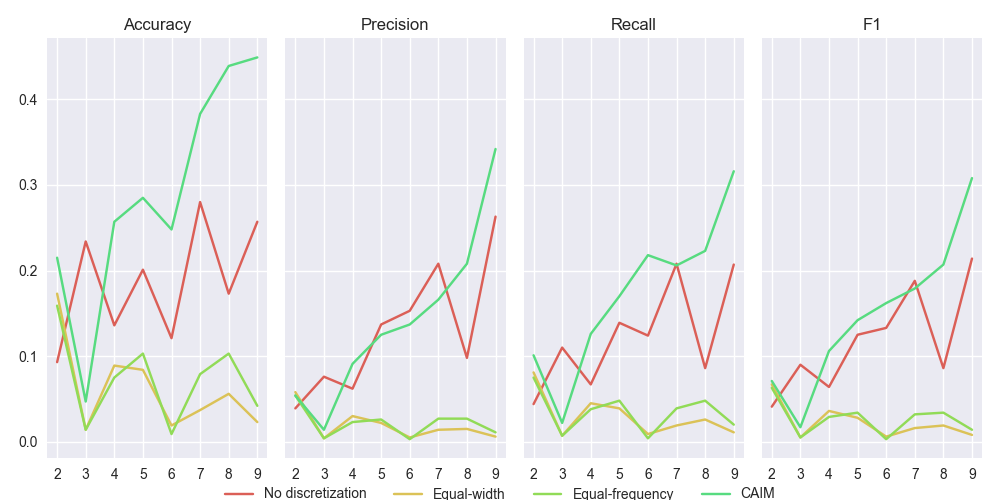
\includegraphics[width=\textwidth]{img/cv_scores_kfold/scoring_kfold_glass.png}
    \caption{Wykresy wartości metryk dla zbioru "Glass" -- kroswalidacja zwykła.}
\end{figure}

Wyniki te również można zaobserwować na przykładzie macierzy konfuzji, gdzie widać, że
klasyfikator słabo spełnia swoje zadanie.
\begin{figure}[H]
\center
    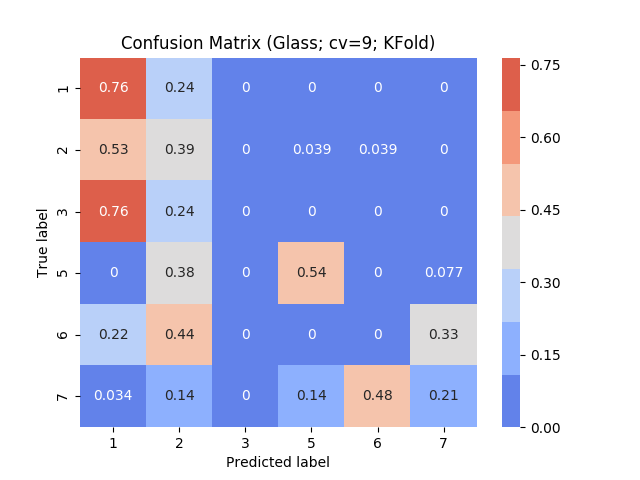
\includegraphics[width=0.6\textwidth]{img/conf_matrices/cm_Glass_cv9_KFold.png}
    \caption{Macierz konfuzji dla najlepszej wartości F1 -- kroswalidacja zwykła.}
\end{figure}

\begin{table}[H]
\center
\caption{Wartości metryk dla zbioru "Glass" -- kroswalidacja zwykła.}
    \begin{tabular}{|c|c|c|c|c|c|c|c|c|c|}
        \hline
        \multirow{2}{*}{\textbf{Metoda dyskr.}} & \multirow{2}{*}{\textbf{Metryka}} & \multicolumn{8}{|c|}{\textbf{CV}} \\ \cline{3-10}
                        &  & 2 & 3 & 4 & 5 & 6 & 7 & 8 & 9 \\ \hline
        \multirow{4}{*}{\textit{Brak}}  & Accuracy & 0.093 & 0.234 & 0.136 & 0.201 & 0.121 & 0.28 & 0.173 & 0.257 \\ \cline{2-10}
                                         & Precision & 0.039 & 0.076 & 0.062 & 0.137 & 0.153 & 0.208 & 0.098 & 0.263 \\ \cline{2-10}
                                         & Recall & 0.044 & 0.11 & 0.067 & 0.139 & 0.124 & 0.208 & 0.086 & 0.207 \\ \cline{2-10}
                                         & F1 & 0.041 & 0.09 & 0.064 & 0.125 & 0.133 & 0.188 & 0.086 & 0.214 \\ \hline \hline


        \multirow{4}{*}{\textit{Equal-width}}  & Accuracy & 0.173 & 0.014 & 0.089 & 0.084 & 0.019 & 0.037 & 0.056 & 0.023 \\ \cline{2-10}
                                                 & Precision & 0.058 & 0.004 & 0.03 & 0.022 & 0.005 & 0.014 & 0.015 & 0.006 \\ \cline{2-10}
                                                 & Recall & 0.081 & 0.007 & 0.045 & 0.039 & 0.009 & 0.019 & 0.026 & 0.011 \\ \cline{2-10}
                                                 & F1 & 0.067 & 0.005 & 0.036 & 0.028 & 0.006 & 0.016 & 0.019 & 0.008 \\ \hline \hline


        \multirow{4}{*}{\textit{Equal-freq}}  & Accuracy & 0.159 & 0.014 & 0.075 & 0.103 & 0.009 & 0.079 & 0.103 & 0.042 \\ \cline{2-10}
                                             & Precision & 0.054 & 0.004 & 0.023 & 0.026 & 0.003 & 0.027 & 0.027 & 0.011 \\ \cline{2-10}
                                             & Recall & 0.075 & 0.007 & 0.038 & 0.048 & 0.004 & 0.039 & 0.048 & 0.02 \\ \cline{2-10}
                                             & F1 & 0.063 & 0.005 & 0.029 & 0.034 & 0.003 & 0.032 & 0.034 & 0.014 \\ \hline \hline


        \multirow{4}{*}{\textit{CAIM}}  & Accuracy & 0.215 & 0.047 & 0.257 & 0.285 & 0.248 & 0.383 & 0.439 & 0.449 \\ \cline{2-10}
                                         & Precision & 0.054 & 0.014 & 0.091 & 0.125 & 0.137 & 0.166 & 0.208 & 0.342 \\ \cline{2-10}
                                         & Recall & 0.101 & 0.022 & 0.126 & 0.17 & 0.218 & 0.206 & 0.223 & 0.316 \\ \cline{2-10}
                                         & F1 & 0.071 & 0.017 & 0.106 & 0.142 & 0.162 & 0.179 & 0.207 & 0.308 \\ \hline \hline
            \hline
        \end{tabular}
    \end{table}